\documentclass[a4paper]{article}
\usepackage{lipsum}
\usepackage{url}
\usepackage{graphicx}
\usepackage{indentfirst}
\usepackage{xcolor}
\usepackage[margin=2cm]{geometry}
\graphicspath{ {images/} }

%Custom Commands
\newcommand{\Pokemon}{Pok\'{e}mon}

%NOTE: 2,000 Words / 4 Pages
%TODO: Also need to do ethics checklist
%TODO: Get a better font and layout :P
%TODO: Think of a better title?
%NOTE: Make the Work Plan codes more detailed
%TODO: Rewrite the Work Plan Descriptions

\begin{document}

%Title Information
\title{
    Project Proposal
    \\ \large{G54IRP/COMP4027}
    \\ \large{Project Title: AI for General Video Game Playing}\vspace{-3ex}}
\author{4262648 Benjamin Charlton (psybc3)}
\date{\vspace{-2ex}12\textsuperscript{th} October 2017}
\maketitle

\section{Background and Motivation}
The following text is filler for now.
\par
\lipsum[1-7]

\section{Aims and Objectives}
This research projects sets out to create and implement a General AI to play video games.
To test and evaluate this goal the solution developed will be tested against the GVGAI framework using the competition rules.\cite{GVGAI2014}
The project will produce an AI to play in the GVGAI framework as well as a research paper describing the performance of the AI created.
\bigbreak
\noindent The objectives of this project are:
\begin{description}
    \item [Background Research]
    Perform research into the current state of AI game playing, general AI, and current well performing solutions to the GVGAI competition.
    The result of this background study will be used to direct the rest of the project and determine a suitable method to tackle the problem with.

    \item [Design a General AI]
    Design an AI suitable to playing general video games as presented in the GVGAI framework.
    The design and approach will be heavily influenced by the research performed earlier in the project, taking account of other previous methods both in and out of the general game playing field as well as how the problem is presented in the framework.

    \item [Develop a General AI]
    Implement and develop the design created to tackle the problem.
    This will be the primary output of the project.
    Due to the heavy reliance on the background research it isn't clear what this stage will involve.

    \item [Evaluation and Analysis of Solution]
    Compare and analyse the performance of the solution against the other entries to the GVGAI competition and potentially against human players.
    If the solution performs well there may be the ability to test them in unseen environments, such as Video Games that aren't shown in the training sets.
\end{description}

\section{Work Plan}
To help outline the project flow and I have created a gantt chart (found in the appendix) and the following descriptions of each portion.

%Explanations of all of the Points on the work plan
\begin{description}
\item [\large{Documentation}]
\item [D1 - Project Proposal Draft]
Write the project proposal draft for approval and feedback from supervisor, due 12\textsuperscript{th} October.
\item [D2 - Project Proposal]
Any revisions to the project proposal that need to be made after supervisor feedback, due 22\textsuperscript{rd} October.
\item [D3 - Preliminary Ethics Checklist]
Fill out and submit the preliminary ethics checklist, no further ethical checks should be required so no further time is scheduled.

\item [Interim Report]
\colorbox{yellow}{Write the interim report summarising the work so far, due 7\textsuperscript{th} December.}
\item [Structure Sections]
\colorbox{yellow}{Decide and begin to structure the sections and the arguments within them for the final dissertation.}
\item [Research Paper]
\colorbox{yellow}{Write the final research paper, due 12\textsuperscript{th} April.}

\item [\large{Research}]
\item [R1 - Research for Proposal]
\colorbox{green}{WRITE THIS}

\item [\large{Development}]
\item [S1 - NEED TO THINK OF THESE]
\colorbox{green}{WRITE THIS}

\item [\large{Presentation}]
\item [P1 - Work on Presentation]
\colorbox{green}{WRITE THIS}
\item [P3 - Create Demo for Presentation]
\colorbox{green}{WRITE THIS}
\item [P3 - Finalise Presentation]
\colorbox{green}{WRITE THIS}
\item [P4 - Present Presentation]
\colorbox{green}{WRITE THIS}

\item [\large{Miscellaneous}]
\item [M1 - Create Git repository]
\colorbox{green}{WRITE THIS}
\item [M3 - Set up LaTeX files]
\colorbox{green}{WRITE THIS}
\item [M3 - SET/SEM Questionaries]
\colorbox{green}{WRITE THIS}

\item [\large{Other Commitments}]
\item [C1 - Welcome Weeks]
First weeks of the academic year, time set aside to allow for settling in as well as running various welcome events.
\item [C2 - Christmas Holiday]
Time off after Autumn term, Partially set aside to all for a break and time to relax..
\item [C3 - Autumn Exams]
Potentially could have exams during the entire 2 weeks so is set aside to allow for revision and the exams themselves.
This can be updated to give a better reflection of when exams will be at a later date.
\item [C4 - Easter Holiday]
Time off after Spring term, As no teaching is happening will give more time to concentrate on coursework and the presentation.
\end{description}

\section{Appendix}
%Bibliography
\bibliography{ProjectProposal}
\bibliographystyle{plain}

%Work Plan
\clearpage
\begin{center}
    \Large{Work Plan}\\
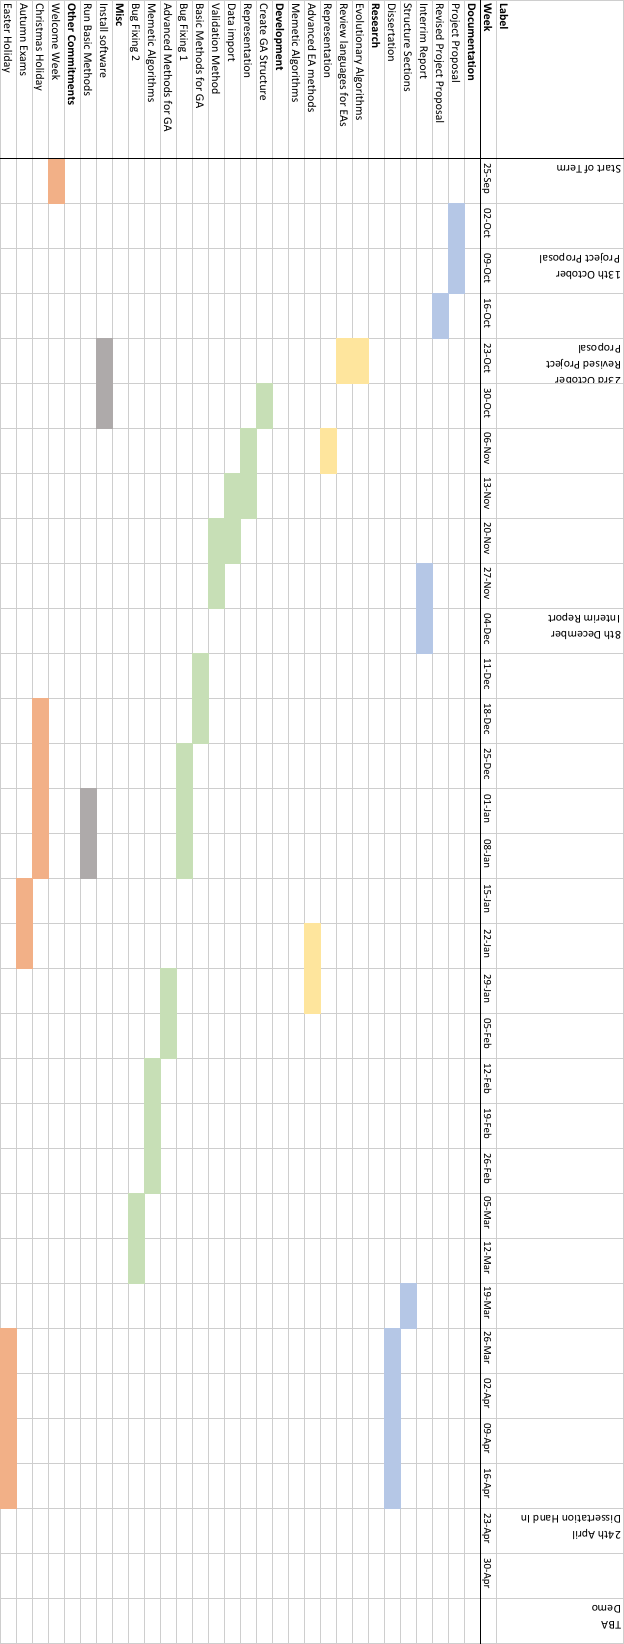
\includegraphics[height=24.8cm]{workPlanOLD.png}
\end{center}


\end{document}
